\SourcePage{322}
\SGAchapter{IX}{Néron 模型与单值性}{Modèles de Néron et monodromie}
\begin{center}A. Grothendieck\\（附 M. Raynaud 所作附录）\end{center}
\textbf{目录}
\begin{enumerate}
\item[0.] 引言。
\item[1.] \Term{abelian-scheme}{阿贝尔概形}的 \Term{neron-model}{Néron 模型}：记号；\Term{canonical-pairing}{典范配对} $\Phi_o\times\Phi'_o\to(\mathbf Q/\mathbf Z)_k$ 与 $(A^\circ,A'{}^\circ)$ 的\Term{canonical-biextension}{典范双扩张} $W^\circ$。
\item[2.] $T_\ell(A_K)$ 的\Term{fixed-part}{固定部分}与\Term{toric-part}{环面部分}。\Term{good-reduction}{好约化}判据。$\ell\ne p$ 时的\Term{orthogonality}{正交}\Term{theorem}{定理}。
\item[3.] \Term{semistable-reduction}{半稳定约化}情形。\Term{semistable-reduction}{半稳定约化}\Term{theorem}{定理}。
\item[4.] 对 Serre--Tate 的一个猜想及\Term{derivation}{导子}的应用。
\item[5.] $\ell=p$ 时的\Term{orthogonality}{正交}\Term{theorem}{定理}（\Term{semistable}{半稳定}情形）。\Term{abelian-scheme}{阿贝尔概形} $B_o$ 与 $B'_o$ 的\Term{duality}{对偶性}。\Term{fixed-part}{固定部分}的刻画。\Term{good-reduction}{好约化}、\Term{potential-good-reduction}{本质好约化}及\Term{semistable-reduction}{半稳定约化}的判据。
\item[6.] 非\Term{semistable-reduction}{半稳定约化}情形下 $T_p(A)$ 的\Term{toric-part}{环面部分}与\Term{fixed-part}{固定部分}的构造的注记。
\item[7.] 与有\Term{semistable-reduction}{半稳定约化}的\Term{abelian-scheme}{阿贝尔概形} $A_K$ 相伴的 $S$ 上 \Term{raynaud-extension}{Raynaud 扩张} $G^\natural$。$S$ 上\Term{abelian-scheme}{阿贝尔概形} $B,B'$ 的\Term{duality}{对偶性}。
\item[8.] \Term{semistable}{半稳定}情形下的 \Term{raynaud-extension}{Raynaud 扩张} $A_K^{\natural\circ}$ 及 ind-群 $A_K^\natural$。
\item[9.] \Term{monodromy-pairing}{单值性配对} $\underline M_\ell\otimes\underline M'_\ell\to\mathbf Z_{\ell S}$ 的定义。
\item[10.] \Term{monodromy-pairing}{单值性配对}的性质。\Term{integrality}{整性}与正性\Term{theorem}{定理}。
\item[11.] \Term{neron-model}{Néron 模型}的\Term{connected-component}{连通分支}：\Term{duality}{对偶}关系与渐近行为。
\end{enumerate}
\SourcePage{323}
\begin{enumerate}
\item[12.] \Term{jacobian}{雅可比簇}的 \Term{neron-model}{Néron 模型}与 \Term{picard-lefschetz-formula}{Picard--Lefschetz 公式}。
\item[13.] 与\Term{transcendental}{超越}理论的联系：复解析情形。13.1 $S$ 上\Term{analytic-group}{解析群}的回顾；13.2 沿一条\Term{fiber}{纤维}的\Term{formal-completion}{形式完备化}；13.3 解析 \Term{raynaud-extension}{Raynaud 扩张}；13.4 用 Deligne 的“\Term{mixed-hodge-structure}{混合 Hodge 结构}”解释；13.5 相对\Term{algebra}{代数}情形。
\item[14.] 与\Term{transcendental}{超越}理论的联系：\Term{rigid-analytic}{刚性解析}情形。\Term{canonical-homomorphism}{典范同态} $\underline M_K\to A_K^{\natural\circ}$。
\end{enumerate}
\SGAsection{0}{引言}
\textbf{0.1.} 本讲把前几讲的结果应用于研究定义在 \Term{henselian}{Hensel} \Term{trait}{离散赋值环谱} $S$ 的\Term{function-field}{函数域} $K$ 上的\Term{abelian-scheme}{阿贝尔概形} $A_K$ 的 \Term{neron-model}{Néron 模型} $A$（1.1）。我们将看到，\Term{neron-model}{Néron 模型}最重要的性质，都可以用\Term{local-monodromy-group}{局部单值群} $I$ 在 \Term{tate-module}{Tate 模} $T_\ell(A_K(\overline K))$ 上的\Term{action}{作用}解释，这里 $\ell$ 是异于 $p$ 的\Term{prime-number}{素数}。由于后者的\Term{dual}{对偶}\Term{solvable}{可解}释为 $\ell$ 进\Term{cohomology-group}{上同调群} $H^1(A_{\overline K},\mathbf Z_\ell)$，而对 $K$ 上每个\Term{projective}{射影}\Term{smooth}{光滑}\Term{scheme}{概形} $X$，$H^1(X_{\overline K},\mathbf Z_\ell)$ 与 $H^1(A_{\overline K},\mathbf Z_\ell)$ 相同，其中 $A_{\overline K}$ 是 $X_{\overline K}$ 的 Albanese \Term{variety}{簇}，所以本讲也可以看作对 $K$ 上\Term{projective}{射影}\Term{smooth}{光滑}\Term{variety}{簇}的 $\ell$ 进 $H^1$（更好地说，“\Term{motive}{动机}的”$H^1$）的\Term{local-monodromy}{局部单值性}现象所作的详细研究。从这个观点看，本讲的主要结果显然应当包含在任意\Term{weight}{权}的\Term{motive}{动机}的“Néron 理论”中，即任意 $i$ 的 $H^i$（$\ell$ 进的、de Rham 的、Hodge 的，等等）的理论中；目前我们才开始窥见这一理论的轮廓。（参见 [9]，尤其是所引报告中 Deligne 的猜想 9.8 至 9.13。）
\SourcePage{324}
\textbf{0.2.} 本讲最重要的结果是“\Term{semistable-reduction}{半稳定约化}\Term{theorem}{定理}”3.6：在把 $K$ 作一个\Term{finite}{有限}\Term{separable-extension}{可分扩张} $K'$ 后，$A_{K'}$ 的\Term{neron-model}{Néron 模型}的\Term{special-fiber}{特殊纤维}的\Term{neutral-component}{单位分支}是一个\Term{abelian-scheme}{阿贝尔概形}被\Term{torus}{环面}的\Term{group-extension}{扩张}。J.-P. Serre 在 1964 年提出了这个猜想，而这里所给证明的基本想法\footnote{这一想法详述于讲者 1964 年 10 月 30 日致 J.-P. Serre 的一封信中。}也可追溯到同一年。我们将看到（3.5），这种“\Term{semistable-reduction}{半稳定约化}”性质\Term{equivalence}{等价}于\Term{monodromy-group}{单值群} $I$ 在 $T_\ell(A_K(\overline K))$ 上的\Term{action}{作用}“本质上为二阶\Term{unipotent}{幺幂}”，其中 $\ell$ 是一个固定的、异于 $S$ 的\Term{residue-characteristic}{剩余特征} $p$ 的\Term{prime-number}{素数}。后一\Term{form}{形式}已经在第 III 讲中用 $\ell$ 进 $H^1$ 作为“\Term{monodromy}{单值性}\Term{theorem}{定理}”的特殊情形得到证明；所用的是二维\Term{excellent-scheme}{优秀概形}的\Term{resolution-of-singularities}{奇点解消}（由 S. Abhyankar 证明）。为建立这两种性质的\Term{equivalence}{等价}性，我们还需要一个“\Term{orthogonality}{正交}\Term{theorem}{定理}”2.4。Igusa [11] 已在如下特殊情形证明了它：$A_K$ 是 $K$ 上\Term{smooth}{光滑}\Term{curve}{曲线} $X_K$ 的\Term{jacobian}{雅可比簇}，而 $X_K$ 是 $S$ 上\Term{projective}{射影}、\Term{regular}{正则}、\Term{connected}{连通}\Term{scheme}{概形} $X$ 的\Term{generic-fiber}{一般纤维}，且其\Term{geometric-special-fiber}{几何特殊纤维}只有普通二次\Term{singular-point}{奇点}。这本身就是\Term{semistable-reduction}{半稳定约化}情形，并不足以满足我们的需要；我们使用前两讲建立的\Term{biextension}{双扩张}理论这一便利工具，主要就是为了证明\Term{generic}{一般}\Term{form}{形式}的\Term{orthogonality}{正交}\Term{theorem}{定理}。顺便指出，D. Mumford 已用他的 $\theta$ 函数理论（未发表）找到了一个完全不同的\Term{semistable-reduction}{半稳定约化}\Term{theorem}{定理}的证明，
\SourcePage{325}
它不用\Term{resolution-of-singularities}{奇点解消}；遗憾的是，他必须把\Term{residue-characteristic}{剩余特征}\Term{restriction}{限制}为异于 $2$。

\textbf{0.3.} \Term{semistable-reduction}{半稳定约化}\Term{theorem}{定理}，是后面各节从“\Term{algebra}{代数}”观点研究 \Term{neron-model}{Néron 模型}的主要工具。最近 D. Mumford 和 M. Raynaud 在 Tate 与 Morikawa 的工作之后，发展了从“\Term{rigid-analytic}{刚性解析}”或“$\theta$ 函数”观点研究 $K$ 上\Term{abelian-variety}{阿贝尔簇}的理论；这个\Term{theorem}{定理}在其中似乎也不可或缺（据说在\Term{complete}{完备}\Term{valued-field}{赋值域}上的\Term{abelian-variety}{阿贝尔簇}问题中，这两个说法是同义的……）。（我们将在第 13、14 节简述\Term{algebra}{代数}观点与\Term{transcendental}{超越}观点之间的联系。）最后，这个\Term{theorem}{定理}还是 Artin--Deligne--Mumford 的“\Term{algebra}{代数}\Term{curve}{曲线}的\Term{semistable-reduction}{半稳定约化}\Term{theorem}{定理}”[3]\footnote{P. Deligne 曾在口头讨论班中证明这个\Term{theorem}{定理}，但没有认为有必要在讨论班文稿中重述。}的证明的关键要素；在研究\Term{fundamental-group}{基本群}上的\Term{monodromy}{单值性}\Term{action}{作用}时，我们已经使用过它（“本质上\Term{tame-action}{温和作用}\Term{theorem}{定理}”，第 V 讲\SGAsourcegap{原书此处在“V”之后留白，未给出具体编号}），本讲的\Term{integrality}{整性}与正性\Term{theorem}{定理} 10.4 的证明中还将再次使用它\footnote{后一个\Term{theorem}{定理}还有一个利用\Term{rigid-analytic}{刚性解析}理论的证明，不使用\Term{semistable-reduction}{半稳定约化}\Term{theorem}{定理}。}。

\textbf{0.4.} 本讲与本讨论班其他各讲的不同之处，在于我们研究 \Term{tate-module}{Tate 模} $T_\ell(A_K)$ 时，系统地兼顾了 $\ell$ 等于\Term{residue-characteristic}{剩余特征} $p$ 的情形。
\SourcePage{326}
\Term{barsotti-tate-group}{Barsotti--Tate 群} [33]\footnote{用 Tate 的术语说，即“\Term{p-divisible-group}{$p$ 可除群}”。}的语言，使得我们可以把 $\ell\ne p$ 时建立的所有最重要的现象推广到这一情形；不过，有时需要使用 Tate 的基本\Term{theorem}{定理} [33，\Term{theorem}{定理} 4]，而该\Term{theorem}{定理}目前只在 $K$ 的\Term{characteristic}{特征}为零时得到证明。当然，在后一情形，\Term{barsotti-tate-group}{Barsotti--Tate pro-$p$ 群} $T_p(A_K)$ 仍可用\Term{monodromy-group}{单值群} $I$ 在 $p$ 进模 $T_p(A_K(\overline K))$ 上的\Term{action}{作用}解释，但须注意，从它与 $\ell\ne p$ 情形的表面类比出发而可能猜想的大多数命题，都严重错误。（例如，$\ell=p$ 时，\Term{monodromy-group}{单值群}的\Term{action}{作用}不再本质上\Term{unipotent}{幺幂}。）然而，若采用更恰当的转述（例如下文 5.13），现在就已清楚：研究以几何方式定义在\Term{residue-characteristic}{剩余特征} $p>0$ 的\Term{trait}{离散赋值环谱}的\Term{function-field}{函数域}上的 \Term{barsotti-tate-group}{Barsotti--Tate pro-$p$ 群}，不论该谱是否为混合\Term{characteristic}{特征}，都应视为“\Term{local-monodromy}{局部单值性}”理论的一部分，其中这些群充当 $\operatorname{Spec}(K)$ 上的“$p$ 进\Term{local-system}{局部系统}”。事实上，它们本质上就是从“$p$ 进”观点研究 $K$ 上\Term{projective}{射影}\Term{smooth}{光滑}\Term{variety}{簇}的 $H^1$ 时出现的“\Term{local-system}{局部系统}”。至于尚待进行的、高次 $H^i$ 的 $p$ 进研究，看起来必须从“\Term{crystalline-cohomology}{晶体上同调}”所提供的观点出发，适当扩大 $K$ 上及 $S$ 上的 \Term{barsotti-tate-group}{Barsotti--Tate pro-$p$ 群}的\Term{category}{范畴}。
\SourcePage{327}
\textbf{0.5.} 本讲直到第 4 节都与口头报告十分接近；后面各节则明显更为详细和\Term{complete}{完备}，原先只作了部分勾勒。后续各讲不使用本讲。反过来，本讲的一些结果（10.4 和 12.5）却使用了将在以后才证明的 \Term{picard-lefschetz-formula}{Picard--Lefschetz 公式}。

\textbf{阅读路线}
\begin{center}
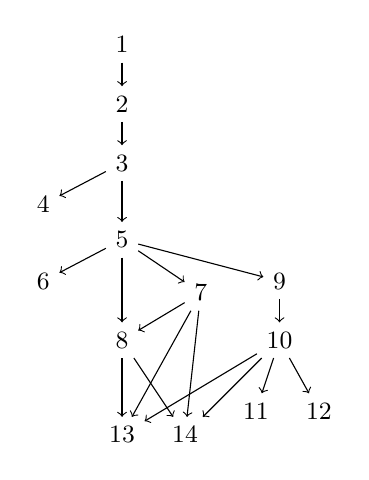
\begin{tikzpicture}[x=1cm,y=.75cm, every node/.style={font=\small}]
\node (a1) at (0,0) {1}; \node (a2) at (0,-1) {2};
\node (a3) at (0,-2) {3}; \node (a4) at (-1,-2.7) {4};
\node (a5) at (0,-3.3) {5}; \node (a6) at (-1,-4) {6};
\node (a7) at (1,-4.2) {7}; \node (a8) at (0,-5) {8};
\node (a9) at (2,-4) {9}; \node (a10) at (2,-5) {10};
\node (a11) at (1.7,-6.2) {11}; \node (a12) at (2.5,-6.2) {12};
\node (a13) at (0,-6.6) {13}; \node (a14) at (.8,-6.6) {14};
\draw[->] (a1)--(a2); \draw[->] (a2)--(a3); \draw[->] (a3)--(a4); \draw[->] (a3)--(a5);
\draw[->] (a5)--(a6); \draw[->] (a5)--(a7); \draw[->] (a5)--(a8); \draw[->] (a5)--(a9);
\draw[->] (a7)--(a8); \draw[->] (a7)--(a13); \draw[->] (a7)--(a14);
\draw[->] (a8)--(a13); \draw[->] (a8)--(a14); \draw[->] (a9)--(a10);
\draw[->] (a10)--(a11); \draw[->] (a10)--(a12); \draw[->] (a10)--(a13); \draw[->] (a10)--(a14);
\end{tikzpicture}
\end{center}
\SourcePage{328}
\SGAsection{1}{阿贝尔概形的 Néron 模型：记号；典范配对 $\Phi_o\times\Phi'_o\to(\mathbf Q/\mathbf Z)_k$ 与 $(A^\circ,A'{}^\circ)$ 的典范双扩张 $W^\circ$}
\textbf{1.0.} 本讲以下始终固定一个\Term{trait}{离散赋值环谱} $S$，并沿用第 I 讲第 1 节中的通常记号 $s,\eta,k,K$ 等。设给定 $K$ 上的\Term{abelian-scheme}{阿贝尔概形} $A_K$，其\Term{dual-abelian-scheme}{对偶阿贝尔概形} [5] 记为 $A'_K$。$A_K$ 与 $A'_K$ 之间的\Term{duality}{对偶性}由 $(A_K,A'_K)$ 上的\Term{divisorial-correspondence}{除子对应} $W_K$ 给出，即 $A_K\times A'_K$ 上的一个相对于 $A_K,A'_K$ 的\Term{unit-section}{单位截面}作了\Term{birigidification}{双刚化}的\Term{invertible-module}{可逆模}；它由其类（见第 VIII 讲 3.1）
\[w_K\in\operatorname{Biext}^1(A_K,A'_K;\mathbf G_{mK})\tag{1.0.1}\]
在唯一\Term{isomorphism}{同构}的意义下唯一确定。与之相应的\Term{pairing}{配对}（第 VIII 讲 2.2）
\[\varphi:T_\ell(A_K)\times T_\ell(A'_K)\longrightarrow\mathbf Z_\ell(1)_K\overset{\mathrm{def}}=T_\ell(\mathbf G_{mK})\tag{1.0.2}\]
将起重要\Term{action}{作用}，其中 $\ell$ 是任意\Term{prime-number}{素数}。当 $\ell\ne p=\operatorname{char}k$ 时，给出 $\varphi$ \Term{equivalence}{等价}于给出\Term{finite-type}{有限型}\Term{free-module}{自由} $\mathbf Z_\ell$ 模的\Term{pairing}{配对}
\[\varphi:T_\ell(A_K(\overline K))\times T_\ell(A'_K(\overline K))\longrightarrow T_\ell(\overline K^*)\tag{1.0.3}\]
并要求它与
\[\pi=\operatorname{Gal}(\overline K/K)\]
在这三个模上的\Term{action}{作用}相容；这里 $\overline K$ 是 $K$ 的\Term{separable-closure}{可分闭包}。已知（第 VIII 讲 3.2）这个\Term{pairing}{配对}是\Term{perfect-duality}{完美对偶}，即把 $T_\ell(A_K(\overline K))$ 和 $T_\ell(A'_K(\overline K))$ 中的每一个，等同于另一个以\Term{invertible-module}{可逆模} $\mathbf Z_\ell(1)=T_\ell(\overline K^*)$ 为值的“\Term{dual}{对偶}”。
\SourcePage{329}
有时我们还假设选定了 $A_K$ 的一个\Term{polarization}{极化}，也就是一个元素
\[\xi\in\operatorname{NS}(A_K/K)=\underline{\operatorname{NS}}_{A_K/K}(K),\tag{1.0.4}\]
其中
\[\underline{\operatorname{NS}}_{A_K/K}\overset{\mathrm{def}}=\underline{\operatorname{Pic}}_{A_K/K}/(\underline{\operatorname{Pic}}^\circ_{A_K/K}=A'_K).\]
它按通常方式定义一个\Term{homomorphism}{同态}
\[\psi_\xi:A_K\longrightarrow A'_K,\tag{1.0.5}\]
从而有一个\Term{homomorphism}{同态}
\[T_\ell(\psi_\xi)\text{ 或 }\psi_\xi:T_\ell(A_K)\longrightarrow T_\ell(A'_K),\tag{1.0.6}\]
以及一个\Term{bilinear-form}{双线性型} $\varphi_\xi$
\[\varphi_\xi(x,y)=\varphi(x,\psi_\xi(y)):T_\ell(A_K)\times T_\ell(A_K)\longrightarrow\mathbf Z_\ell(1)_K.\tag{1.0.7}\]
当 $\ell\ne p$ 时，也可以把它解释为带\Term{action}{作用}的\Term{finite-type}{有限型}\Term{free-module}{自由} $\mathbf Z_\ell$ 模的\Term{pairing}{配对}：
\[\varphi_\xi:T_\ell(A_K(\overline K))\times T_\ell(A_K(\overline K))\longrightarrow T_\ell(\overline K^*).\tag{1.0.8}\]
这些构造对 $A_K$ 的 Néron--Severi \Term{group}{群}中的任意元素都有意义，所得的型 $\varphi_\xi$，即 (1.0.7) 或 (1.0.8)，是\Term{alternating}{交错}的（第 VIII 讲 2.2.11）。$\xi$ 是\Term{polarization}{极化}，蕴含 (1.0.5) 中的 $\psi_\xi$ 是一个\Term{isogeny}{同源}；由于 $\dim A_K=\dim A'_K$，这又\Term{equivalence}{等价}于它是\Term{group}{群}的\Term{epimorphism}{满态射}，也\Term{equivalence}{等价}于 (1.0.6) 中的 $T_\ell(\psi_\xi)$ 是\Term{injective}{单射}（或\Term{equivalence}{等价}地，有\Term{finite}{有限}\Term{cokernel}{余核}），最后还\Term{equivalence}{等价}于 (1.0.7) 的型 $\varphi_\xi$ 是\Term{separating}{分离的}。
\SourcePage{330}
\textbf{1.1.} 回顾一下，$S$ 上存在一个\Term{smooth}{光滑}\Term{scheme}{概形} $A$，称为 $A_K$ 的 \Term{neron-model}{Néron 模型}，它\Term{representable}{表示}定义在\Term{smooth}{$S$ 上光滑}\Term{scheme}{概形}的\Term{category}{范畴}上的\Term{functor}{函子}
\[S'\longmapsto\operatorname{Hom}_\eta(S'_\eta,A_\eta).\tag{1.1.1}\]
因此，按照定义，对 $S$ 上的相对\Term{smooth}{光滑}\Term{scheme}{概形} $S'$，有关于 $S'$ 的\Term{functor}{函子}\Term{isomorphism}{同构}
\[\operatorname{Hom}_S(S',A)\xrightarrow\sim\operatorname{Hom}_\eta(S'_\eta,A_\eta).\tag{1.1.2}\]
当 $S$ 的\Term{residue-field}{剩余域} $k$ 是\Term{perfect-field}{完美域}时，Néron [19] 给出了 $A$ 的构造；Raynaud 在 1966/67 年于 IHÉS 主讲的一个未整理成文的讨论班中，把它推广到\Term{generic}{一般}情形（Raynaud 得到的主要结果的陈述见 [21]，这些结果补充了 Néron 在上述文献中的结果）。这里我们承认这个存在性结果，也承认 $A$ 是 $S$ 上的\Term{quasi-projective}{拟射影}\Term{scheme}{概形}。对 $\eta$ 上\Term{smooth}{光滑}的 $S'$ 应用 (1.1.2)，还可看出下列\Term{canonical-morphism}{典范态射}是\Term{isomorphism}{同构}：
\[A\times_S\operatorname{Spec}(K)\xrightarrow\sim A_K.\tag{1.1.3}\]
这说明成对使用记号 $A,A_K$ 是合理的。必要时也以 $A_\eta$ 代替 $A_K$。把 (1.1.3) 用作等同\Term{isomorphism}{同构}，则\Term{canonical}{典范}\Term{bijection}{双射} (1.1.2) 正是\Term{restriction}{限制}到\Term{generic-fiber}{一般纤维}的映射。

由于\Term{functor}{函子} (1.1.1) 显然带有\Term{commutative-group}{交换群}结构，所以\Term{representable}{表示}它的 \Term{neron-model}{Néron 模型} $A$ 自身也带有 $S$ 上\Term{smooth}{光滑}\Term{commutative-group-scheme}{交换群概形}的结构。本讲以下的内容专门研究这个\Term{group-scheme}{群概形}。
\SourcePage{331}
考虑 \Term{neron-model}{Néron 模型}自然得到的一个重要\Term{invariant}{不变量}，是 $k$ 上\Term{smooth}{光滑}\Term{finite-type}{有限型}的\Term{commutative-group-scheme}{交换群概形}
\[A_o=A\times_Ss=A_k.\tag{1.1.4}\]
按\Term{generic}{一般}记号，以 $A_o^\circ$ 表示其\Term{neutral-component}{单位分支}，并考虑 $A_o$ 的\Term{connected-component-group}{连通分支群}\Term{scheme}{概形}
\[\Phi_o=A_o/A_o^\circ,\tag{1.1.5}\]
它是 $k$ 上的\Term{finite}{有限}\Term{etale}{平展}\Term{group-scheme}{群概形}。用 $k$ 的\Term{separable-closure}{可分闭包} $\overline k$ 来说，它由通常意义下的\Term{finite}{有限}\Term{group}{群}
\[\Phi_o(\overline k)\tag{1.1.6}\]
及
\[\pi_o=\operatorname{Gal}(\overline k/k)\]
在这个\Term{group}{群}上的自然\Term{action}{作用}确定。

我们将同时研究 $A_K$ 的 \Term{neron-model}{Néron 模型} $A$ 以及
\[A'=A'_K\text{ 的 Néron 模型},\tag{1.1.7}\]
后者也是 $S$ 上\Term{smooth}{光滑}\Term{finite-type}{有限型}的\Term{commutative-group-scheme}{交换群概形}。以
\[\Phi'_o=A'_o/A'_o{}^\circ\tag{1.1.8}\]
表示其\Term{special-fiber}{特殊纤维} $A_o$ 的\Term{connected-component-group}{连通分支群}。
\SourcePage{332}
\textbf{1.2.} 对 $(A,A')$ 以及 (1.0.1) 中 $(A_K,A'_K)$ 被 $\mathbf G_{mK}$ 的\Term{biextension}{双扩张} $W_K$ 应用第 VIII 讲 7.1 b)，得到\Term{canonical}{典范}\Term{pairing}{配对}
\[\Phi_o\times\Phi'_o\longrightarrow(\mathbf Q/\mathbf Z)_k,\tag{1.2.1}\]
即 $\pi_o$ 模的\Term{pairing}{配对}
\[\Phi_o(\overline k)\times\Phi'_o(\overline k)\longrightarrow\mathbf Q/\mathbf Z.\tag{1.2.2}\]
这里，这个\Term{pairing}{配对}\Term{presentation}{表现}为把 $W_K$ 延拓成 $(A,A')$ 被 $\mathbf G_{mS}$ 的\Term{biextension}{双扩张} $W$ 的\Term{obstruction}{障碍}；第 VIII 讲 7.3.2 详细说明了这一观点的意义。关于这个\Term{pairing}{配对}，先提出如下猜想。
\begin{SGAresult}{猜想}{1.3}
\Term{pairing}{配对} (1.2.1) 是\Term{perfect-duality}{完美对偶}，即把\Term{connected-component-group}{连通分支群} $\Phi_o$ 与 $\Phi'_o$ 中的每一个等同于另一个以 $(\mathbf Q/\mathbf Z)_k$ 为值的\Term{dual}{对偶}。
\end{SGAresult}
\textbf{1.3.1.} 由 (1.2.1) 的形成与\Term{form}{形式}\Term{net}{净}\Term{base-change}{基变换}交换（第 VIII 讲 7.3.5.3），以及 \Term{neron-model}{Néron 模型}的形成的类似性质可知，只需在 $S$ \Term{complete}{完备}且\Term{residue-field}{剩余域}\Term{separably-closed}{可分闭}的情形证明 1.3。Artin 与 Mazur 已在 $A_K$ 是 $K$ 上\Term{proper}{固有}\Term{smooth}{光滑}\Term{curve}{曲线}的\Term{jacobian}{雅可比簇}时，利用他们关于 $S$ 上\Term{proper}{固有}\Term{curve-scheme}{曲线概形}的相对\Term{jacobian}{雅可比簇}的\Term{self-duality}{自对偶性}的\Term{generic}{一般}理论（未发表，在\Term{derived-category}{导出范畴}意义下）证明了这个猜想；当\Term{residue-field}{剩余域}为\Term{finite-field}{有限域}时，他们又利用 Tate 的\Term{duality}{对偶性}理论 [32] 证明了同一个猜想 1.3。我们还将在 11.4 与 11.5 看到（略去一些相容性的核对），
\SourcePage{333}
1.3 对异于 $p$ 的 $\ell$ 的 $\ell$ \Term{primary-component}{准素部分}成立，而且在“\Term{semistable-reduction}{半稳定约化}”情形成立。这些结果使 1.3 极为可信。还可以把 1.3 看作\Term{complete}{完备}\Term{discrete-valuation-ring}{离散赋值环}的\Term{fraction-field}{分式域}上的\Term{group-scheme}{群概形}的\Term{generic}{一般}\Term{duality}{对偶性}理论的副产物；这一理论在\Term{form}{形式}上类似于 SGA 5 第 I 讲的理论，目前仍停留在启发性阶段，并且还应包含 Serre [27] 所给\Term{form}{形式}的\Term{local-scheme}{局部}\Term{class-field-theory}{类域论}。

\textbf{1.3.2.} 对给定的\Term{abelian-scheme}{阿贝尔概形} $A_K$ 而言，1.3 成立\Term{equivalence}{等价}于\Term{pairing}{配对} (1.2.1) 在左、右两边都\Term{separating}{分离}。由第 VIII 讲 7.3.2，它在左边\Term{separating}{分离}，意味着 $A$ 的满足下述条件的唯一\Term{open-subgroup-scheme}{开子群概形} $V$ 是 $A$ 的\Term{neutral-component}{单位分支} $A^\circ$：$W_K$ 可延拓成 $(V,A')$ 被 $\mathbf G_{mS}$ 的\Term{biextension}{双扩张}。对 (1.2.1) 在右边\Term{separating}{分离}的条件也有\Term{symmetric}{对称}的解释。

\textbf{1.4.} \Term{generic}{一般}地，设
\[U\subset A\quad\text{及}\quad U'\subset A'\tag{1.4.1}\]
是\Term{open-subgroup-scheme}{开子群概形}，使得 $W_K$ 可延拓为 $(U,U')$ 被 $\mathbf G_{mS}$ 的\Term{biextension}{双扩张}（由第 VIII 讲 7.3.2，这可以明确表述为：$U,U'$ 所定义的 $\Phi_o,\Phi'_o$ 的\Term{subgroup}{子群}
\[\Psi_o=U_o/U_o^\circ\subset\Phi_o,\qquad\Psi'_o=U'_o/U'_o{}^\circ\subset\Phi'_o\tag{1.4.2}\]
关于\Term{pairing}{配对} (1.2.1) 相互\Term{orthogonality}{正交}），
\SourcePage{334}
则以 $W$ 表示 $W_K$ 的这个延拓（它在唯一\Term{isomorphism}{同构}的意义下唯一）。它由其类
\[w\in\operatorname{Biext}^1(U,U';\mathbf G_{mS})\tag{1.4.3}\]
在唯一\Term{isomorphism}{同构}的意义下确定，而这个类又由其在 $\operatorname{Biext}^1(A_K,A'_K;\mathbf G_{mK})$ 中的像是 (1.0.1) 的 $w_K$ 这一条件刻画。

例如，可以取 $U,U'$ 为 $A,A'$ 的\Term{neutral-component}{单位分支} $A^\circ,A'{}^\circ$。由此得到 $(A^\circ,A'{}^\circ)$ 被 $\mathbf G_{mS}$ 的\Term{canonical}{典范}\Term{biextension}{双扩张} $W^\circ$ 或 $W$，及其类
\[w=w^\circ\in\operatorname{Biext}^1(A^\circ,A'{}^\circ;\mathbf G_{mS});\tag{1.4.4}\]
我们主要将使用它。显然，对各种 $(U,U')$ 而言，类 $w$ (1.4.3) \Term{restriction}{限制}到 $(A^\circ,A'{}^\circ)$ 上都等于 $w^\circ$ (1.4.4)。
\begin{SGAresult}{命题}{1.5}
考虑 $(A^\circ,A'{}^\circ)$ 被 $\mathbf G_{mS}$ 的\Term{canonical}{典范}\Term{biextension}{双扩张} (1.4.4) $W$ 的\Term{special-fiber}{特殊纤维} $W_s$；于是 $W_s$ 是 $(A_o^\circ,A'_o{}^\circ)$ 被 $\mathbf G_{mk}$ 的\Term{biextension}{双扩张}。这个\Term{biextension}{双扩张}是\Term{separating}{分离的}（第 VIII 讲 4.11）。
\end{SGAresult}
\begin{proof}
在 $A^\circ$ 上选取一个\Term{ample}{丰沛}\Term{invertible-module}{可逆模} $L$。于是 $L_\eta$ 定义一个\Term{homomorphism}{同态}（见 1.0.5）
\[A_K\longrightarrow A'_K,\]
它延拓为\Term{homomorphism}{同态} $A\to A'$，因而给出
\[\psi:A^\circ\longrightarrow A'{}^\circ;\]
可以考虑 $(A^\circ,A^\circ)$ 被 $\mathbf G_{mS}$ 的\Term{biextension}{双扩张} $W_L$，即 $W$ 沿 $(\operatorname{id}_{A^\circ},\psi)$ 的\Term{inverse-image}{逆像}。
\SourcePage{335}
$W_L$ 在\Term{generic-fiber}{一般纤维}上的\Term{restriction}{限制}，正是第 VIII 讲 4.12 中的\Term{biextension}{双扩张} $\delta(L_\eta)$。因此由第 VIII 讲 7.4，$W_L$ 对应于\Term{birigidification}{双刚化}的\Term{invertible-module}{可逆模} $\delta(L)$，从而 $(W_L)_s$ 由 $\delta(L_s)$ 定义。另一方面，也可把它描述为\Term{biextension}{双扩张} $W_s$ 沿\Term{morphism}{态射}
\[\operatorname{id}_{A_o^\circ}:A_o^\circ\longrightarrow A_o^\circ,\qquad\psi_o:A_o^\circ\longrightarrow A'_o{}^\circ\]
的\Term{inverse-image}{逆像}。因为 $L_s$ \Term{ample}{丰沛}，由第 VIII 讲 4.13，$W_{L_s}$ \Term{separating}{分离}，特别是在左边\Term{separating}{分离}，所以 $W_s$ 更在左边\Term{separating}{分离}。由\Term{symmetry}{对称性}，$W_s$ 在右边也\Term{separating}{分离}，这就证明了 1.5。
\end{proof}
指出，当 $A_o^\circ$ 的\Term{unipotent-rank}{幺幂秩}为零时，我们将把 1.5 大大精确化（5.4）。

\SGAsection{2}{$T_\ell(A_K)$ 的固定部分与环面部分。好约化判据。$\ell\ne p$ 时的正交定理}
\textbf{2.1.} 与 $k$ 上任意\Term{commutative-algebraic-group}{交换代数群}一样，$A_o$ 有一个最大的\Term{subtorus}{子环面}，其形成与\Term{base-field}{基域}的任意\Term{extension}{扩张}交换 [SGA 3，第 XVII 讲 7.2.1，第 XII 讲 1.12]：
\[T_o\subset A_o.\tag{2.1.1}\]
当 $k$ 是\Term{perfect-field}{完美域}时，$T_o$ 由下述条件刻画：$A_o^\circ/T_o$ 是 $k$ 上一个\Term{abelian-scheme}{阿贝尔概形} $B_o$ 被一个（\Term{smooth}{光滑}\Term{connected}{连通}）\Term{unipotent-group}{幺幂群}的\Term{group-extension}{扩张} [25]；这个\Term{unipotent-group}{幺幂群}必有一个各商均\Term{isomorphism}{同构}于 $\mathbf G_{ak}$ 的\Term{composition-series}{合成列}（SGA 3，第 XVII 讲 4.1.3）：
\SourcePage{336}
\[0\longrightarrow U_o\longrightarrow A_o^\circ/T_o\longrightarrow B_o\longrightarrow0.\tag{2.1.2}\]
无论 $k$ \Term{perfect}{完美}与否，若 $A_o^\circ$ 是一个\Term{abelian-scheme}{阿贝尔概形} $B_o$ 被一个\Term{affine}{仿射}\Term{smooth}{光滑}\Term{connected}{连通}\Term{scheme}{概形} $L_o$ 的\Term{group-extension}{扩张}：
\[0\longrightarrow L_o\longrightarrow A_o^\circ\longrightarrow B_o\longrightarrow0,\tag{2.1.3}\]
则已知这个\Term{group-extension}{扩张}结构唯一 [25]，而且此时 $T_o\subset L_o$，故 $T_o$ 是 $L_o$ 的最大\Term{subtorus}{子环面}，从而有\Term{exact-sequence}{正合列} (2.1.2)，其中
\[U_o=L_o/T_o.\tag{2.1.4}\]
\textbf{2.1.5.} 指出，$A_o^\circ$ 的\Term{unipotent-rank}{幺幂秩}为零（即在 $k$ 的一个\Term{algebraic-closure}{代数闭包}上，它没有\Term{isomorphism}{同构}于 $\mathbf G_a$ 的\Term{subgroup}{子群}），当且仅当 $A_o^\circ/T_o$ 是一个\Term{abelian-scheme}{阿贝尔概形} $B_o$；这时前面的条件成立，且 $U_o=0$。

若 $\ell$ 是异于 $k$ 的\Term{characteristic}{特征}的\Term{prime-number}{素数}，因而 $A_o^\circ$ 为 $\ell$ \Term{divisible}{可除}，则包含 (2.1.1) 给出 pro-\Term{group-scheme}{群概形}的\Term{exact-sequence}{正合列}
\[
\begin{tikzcd}[column sep=small]
0\arrow[r]&T_\ell(T_o)\arrow[r]&T_\ell(A_o^\circ)\arrow[r]\arrow[d,"\wr"']&T_\ell(A_o^\circ/T_o)\arrow[r]\arrow[d,"\wr"']&0\\
&&T_\ell(A_o)&T_\ell(A_o/T_o)&
\end{tikzcd}\tag{2.1.6}
\]
其中各项也可以解释为自由\Term{twisted-constant-sheaf}{扭常值} $\ell$ 进\Term{sheaf}{层}。当有\Term{exact-sequence}{正合列} (2.1.2) 时，例如 $k$ \Term{perfect}{完美}或 $A_o^\circ$ 的\Term{unipotent-rank}{幺幂秩}为零时，就有
\[T_\ell(A_o^\circ/T_o)\xrightarrow\sim T_\ell(B_o),\tag{2.1.7}\]
\SourcePage{337}
因而\Term{exact-sequence}{正合列} (2.1.5) 此时写成
\[0\longrightarrow T_\ell(T_o)\longrightarrow T_\ell(A_o^\circ)\longrightarrow T_\ell(B_o)\longrightarrow0.\tag{2.1.8}\]
置
\[n=\dim A_K=\dim A_o,\quad\mu=\dim T_o,\quad\lambda=\dim U_o,\quad\alpha=\dim B_o;\tag{2.1.9}\]
于是
\[n=\mu+\lambda+\alpha,\tag{2.1.10}\]
\[\begin{cases}
\operatorname{rank}T_\ell(T_o)=\mu,\quad\operatorname{rank}T_\ell(A_o^\circ/T_o)=\operatorname{rank}T_\ell(B_o)=2\alpha,\\
\operatorname{rank}T_\ell(A_o^\circ)=\mu+2\alpha.
\end{cases}\tag{2.1.11}\]
第二个关系是 Weil 的一个著名\Term{theorem}{定理} [5] [15]。

\textbf{2.1.12.} 即使不假定有\Term{exact-sequence}{正合列} (2.1.2)，通过转到 $k$ 的一个\Term{algebraic-closure}{代数闭包}，整数 $n,\mu,\lambda,\alpha$ 显然也有定义；它们分别称为 $A_o$ 的\Term{dimension}{维数}、$A_o$ 的\Term{reductive-rank}{约化秩}（即 $T_o$ 的\Term{dimension}{维数}）、$A_o$ 的\Term{unipotent-rank}{幺幂秩}、$A_o$ 的\Term{abelian-rank}{阿贝尔秩}。它们仍满足关系 (2.1.10) 与 (2.1.11)（在后者中略去 $\operatorname{rank}T_\ell(B_o)$ 一项……）。

\textbf{2.1.13.} 当 $k$ 的\Term{characteristic}{特征}为 $p>0$，且 $A_o^\circ$ 是 $p$ \Term{divisible}{可除}的，或\Term{equivalence}{等价}地，其\Term{unipotent-rank}{幺幂秩}为零（见 2.1.5）时，也应考虑 pro-\Term{group}{群} $T_p(A_o^\circ)$，它是一个\Term{barsotti-tate-group}{Barsotti--Tate 群}（用 [33] 的术语说，是一个\Term{p-divisible-group}{$p$ 可除群}）。此时\Term{exact-sequence}{正合列} (2.1.8) 对 $\ell=p$ 仍然成立，而且是\Term{barsotti-tate-group}{Barsotti--Tate 群}的\Term{exact-sequence}{正合列}。这里 $\lambda=0$，所以
\[n=\mu+\alpha,\tag{2.1.13.1}\]
\SourcePage{338}
公式 (2.1.11) 也仍然成立，只须将其中的\Term{rank}{秩}解释为相应\Term{barsotti-tate-group}{Barsotti--Tate 群}的\Term{rank}{秩}（或“\Term{height}{高度}”）。

\textbf{2.1.14.} 对 $A'_o{}^\circ$ 同样引入\Term{invariant}{不变量}
\[T'_o\subset A'_o{}^\circ,\qquad U'_o,\qquad B'_o,\]
其中 $T'_o$ 是 $A'_o{}^\circ$ 的\Term{toric-part}{环面部分}，$B'_o$ 是其\Term{abelian-part}{阿贝尔部分}（特别在 $k$ \Term{perfect}{完美}或 $A'_o{}^\circ$ 的\Term{unipotent-rank}{幺幂秩}为零时有定义），$U'_o$ 是其\Term{unipotent-part}{幺幂部分}（例如 $k$ \Term{perfect}{完美}时有定义，而 $A'_o{}^\circ$ 的\Term{unipotent-rank}{幺幂秩}为零时也显然有定义）。得到相应于 (2.1.6) 或 (2.1.8) 的\Term{exact-sequence}{正合列}，这里不再写出。也可以像 (2.1.9) 那样为 $A'_o{}^\circ$ 引入整数 $\mu',\lambda',\alpha'$，但下文（2.2.7）将说明，它们与 $A_o^\circ$ 的相同，因而不必再为它们引入新的记号。

\textbf{2.2.} 我们拟借助 $T_\ell(A^\circ)$，精确说明 $T_\ell(A_K)$ 与 $T_\ell(A_o)=T_\ell(A_o^\circ)$ 之间的关系。先回顾：
\begin{SGAresult}{\Term{lemma}{引理}}{2.2.1}
设 $m>0$ 为整数。下列条件\Term{equivalence}{等价}：
\begin{enumerate}
\item[(i)] $m\operatorname{id}_{A^\circ}$ \Term{flat}{平坦}。
\item[(ii)] $m\operatorname{id}_{A^\circ}$ \Term{surjective}{满射}。
\item[(iii)] $m\operatorname{id}_{A^\circ}$ \Term{quasi-finite}{拟有限}。
\item[(iv)] $m$ 与 $k$ 的\Term{characteristic}{特征}互素，或 $A_o^\circ$ 的\Term{unipotent-rank}{幺幂秩}为零（见 1.5.5）。
\end{enumerate}
此外，若上述条件对 $m$ 成立，则对每个 $\nu>0$，它们也对 $m^\nu$ 成立；\Term{group}{群}
\SourcePage{339}
\[{}_{m^\nu}A^\circ\overset{\mathrm{def}}=\operatorname{Ker}(m^\nu\operatorname{id}_{A^\circ})\]
在 $S$ 上\Term{quasi-finite}{拟有限}、\Term{separated}{分离}且\Term{flat}{平坦}，并随 $\nu$ 组成一个\Term{group-scheme}{群概形}的\Term{projective-system}{投射系}，其转移\Term{morphism}{态射}
\[x\longmapsto m^{\nu'-\nu}x:\quad{}_{m^{\nu'}}A^\circ\longrightarrow{}_{m^\nu}A^\circ\]
\Term{faithfully-flat}{忠实平坦}。
\end{SGAresult}
\begin{proof}
\Term{fiber}{纤维}\Term{flatness}{平坦性}判据（EGA IV 11.3.5）说明，(i) 与 (ii)、(iii) 一样都是\Term{fiber}{纤维}上的条件；由于所考虑的\Term{fiber}{纤维}都\Term{smooth}{光滑}\Term{connected}{连通}，由 SGA 3 第 VI$_A$ 讲 5.6，这些条件彼此\Term{equivalence}{等价}。从\Term{form}{形式} (ii) 以及 Weil 的一个经典\Term{theorem}{定理} [5] [15] 又可看出，这些条件在\Term{generic-fiber}{一般纤维}上成立，因为后者是\Term{abelian-scheme}{阿贝尔概形}，所以只须将它在\Term{special-fiber}{特殊纤维}上表达出来。由结构理论，它与 (iv) 的\Term{equivalence}{等价}性也是熟知的。无论采用哪种\Term{form}{形式}，该条件在 $m\mapsto m^\nu$ 下保持显然成立；因此这些条件蕴含 ${}_{m^\nu}A^\circ$ 是 $S$ 上\Term{flat}{平坦}\Term{quasi-finite}{拟有限}的\Term{group-scheme}{群概形}，并且显然在 $S$ 上\Term{separated}{分离}，因为 $A^\circ$ 本身\Term{separated}{分离}。最后，关于所考虑的转移\Term{morphism}{态射}的\Term{faithfully-flat}{忠实平坦性}的断言，\Term{equivalence}{等价}于说它们对 fppf \Term{topology}{拓扑}是\Term{epimorphism}{满态射}；这由 $m\operatorname{id}_{A^\circ}$ \Term{faithfully-flat}{忠实平坦}，从而对该\Term{topology}{拓扑}是\Term{epimorphism}{满态射}，\Term{form}{形式}地\Term{pushout}{推出}。
\end{proof}
\textbf{2.2.2.} 以下取 $m$ 为满足 2.2.1 的条件的\Term{prime-number}{素数} $\ell$。以
\[T_\ell(A^\circ)=({}_{\ell^\nu}A^\circ)_{\nu>0}\tag{2.2.2.1}\]
表示 2.2.1 所描述的\Term{projective-system}{投射系}。
\SourcePage{340}
注意，经由两个\Term{base-change}{基变换} $\eta\to S$ 及 $s\to S$，它分别给出 1.0 和 2.1 中考虑的\Term{projective-system}{投射系} $T_\ell(A_K)$ 与 $T_\ell(A_o^\circ)=T_\ell(A_o)$。

\textbf{2.2.3.} 现在假设 $S$ 为\Term{henselian}{Hensel 的}。已知，$S$ 上每个\Term{quasi-finite}{拟有限}\Term{separated}{分离}\Term{scheme}{概形} $X$ 均\Term{canonical-decomposition}{典范分解}为和
\[X=X^f\amalg X',\tag{2.2.3.1}\]
其中 $X^f$ 在 $S$ 上\Term{finite}{有限}，而 $X'_o=\varnothing$，即 $X'$ 只有它的\Term{generic-fiber}{一般纤维} $X'_\eta$；所以 $X^f$ 与 $X$ 的\Term{special-fiber}{特殊纤维}相同。这个\Term{resolution}{分解}显然对 $X$ 具有\Term{functoriality}{函子性}。特别地，由此可知，若 $X$ 是 $S$ 上的\Term{group-scheme}{群概形}，则 $X^f$ 是它的\Term{subgroup-scheme}{子群概形}。若 $X$ 在 $S$ 上\Term{flat}{平坦}（或\Term{etale}{平展}），则 $X^f$ 显然也如此。

把这应用于 $T_\ell(A^\circ)$ 的各\Term{set-component}{分量} ${}_{\ell^\nu}A^\circ$，得到\Term{group}{群}的一个子\Term{projective-system}{投射系}
\[\bigl(({}_{\ell^\nu}A^\circ)^f\bigr)_{\nu>0}\overset{\mathrm{def}}=T_\ell(A^\circ)^f\subset T_\ell(A^\circ),\tag{2.2.3.2}\]
称为 \Term{tate-module}{Tate 模} $T_\ell(A^\circ)$ 的\Term{fixed-part}{固定部分}。由构造，显然有对 $A$ 具有\Term{functoriality}{函子性}的\Term{canonical-isomorphism}{典范同构}
\[T_\ell(A^\circ)^f\times_Ss\xrightarrow\sim T_\ell(A^\circ)\times_Ss\xrightarrow\sim T_\ell(A_o^\circ).\tag{2.2.3.3}\]
另一方面，$T_\ell(A^\circ)^f$ 的\Term{generic-fiber}{一般纤维}定义了 $T_\ell(A_K)$ 的一个\Term{canonical}{典范}子 pro-\Term{group}{群}，仍称为这个 \Term{tate-module}{Tate 模}的“\Term{fixed-part}{固定部分}”，记为
\[T_\ell(A_K)^f\subset T_\ell(A_K).\tag{2.2.3.4}\]
\SourcePage{341}
\textbf{2.2.4.} 当 $\ell\ne p=\operatorname{char}k$ 时，$T_\ell(A^\circ)^f$ \Term{solvable}{可解}释为 $S$ 上的\Term{twisted-constant-sheaf}{扭常值} $\ell$ 进\Term{sheaf}{层}（各 ${}_{\ell^\nu}A^\circ$ 在 $S$ 上\Term{finite}{有限}\Term{etale}{平展}）。由于 $S$ 为\Term{henselian}{Hensel 的}，\Term{functor}{函子}
\[X\longmapsto X_o=X\times_Ss\]
从 $S$ 上\Term{finite}{有限}\Term{etale}{平展}\Term{scheme}{概形}的\Term{category}{范畴}到 $k$ 上\Term{finite}{有限}\Term{etale}{平展}\Term{scheme}{概形}的\Term{category}{范畴}是一个\Term{equivalence-of-categories}{范畴等价}；因此，$S$ 上和 $k$ 上\Term{twisted-constant-sheaf}{扭常值} $\ell$ 进\Term{sheaf}{层}的\Term{category}{范畴}之间，也有类似的\Term{equivalence-of-categories}{等价}。所以给出 $T_\ell(A^\circ)^f$ 的\Term{special-fiber}{特殊纤维}的关系 (2.2.3.3)，在唯一\Term{isomorphism}{同构}的意义下刻画了这个\Term{fixed-part}{固定部分}。另一方面，作为 $T_\ell(A^\circ)$ 的 $\ell$ 进\Term{subsheaf}{子层}，它显然由其\Term{generic-fiber}{一般纤维} (2.2.3.4) 刻画，\Term{equivalence}{等价}地，由相应的、在 $\pi=\operatorname{Gal}(\overline K/K)$ 下\Term{stable}{稳定}的 $\mathbf Z_\ell$ \Term{submodule}{子模}刻画：
\[T_\ell(A_K)^f(\overline K)\overset{\mathrm{def}}=T_\ell(A(\overline K))^f\subset T_\ell(A(\overline K)).\tag{2.2.4.1}\]
事实上，有以下结果。
\begin{SGAresult}{命题}{2.2.5}
仍设 $\ell\ne p$，且 $S$ 为\Term{henselian}{Hensel 的}。则 $T_\ell(A(\overline K))=T_\ell(A_K)(\overline K)$ 中对应于 $T_\ell(A_K)$ 的\Term{fixed-part}{固定部分} $T_\ell(A_K)^f$ (2.2.3.4) 的\Term{submodule}{子模} (2.2.4.1)，就是\Term{inertia-group}{惯性群} $I\subset\pi$ 下的\Term{invariant-submodule}{不变子模} $T_\ell(A(\overline K))^I$。
\end{SGAresult}
\begin{proof}
这将由对下列类似关系取\Term{projective-limit}{投射极限}得到；该关系对每个与 $p=\operatorname{char}k$ 互素的整数 $m>0$ 都成立：
\[({}_mA)^f(\overline K)=({}_mA(\overline K))^I.\tag{2.2.5.1}\]
\SourcePage{342}
为证明这个关系，引入 $S$ 的\Term{strict-localization}{严格局部化} $\widetilde S$，其\Term{fraction-field}{分式域} $\widetilde K$ 是 $\overline K/K$ 的最大\Term{unramified-extension}{非分歧子扩张}。由于 $({}_mA)^f$ 在 $S$ 上\Term{finite}{有限}\Term{etale}{平展}，它的 $\overline K$ 值点已经是 $\widetilde K$ 值点，所以 (2.2.5.1) 的左边正是 $\operatorname{Hom}_S(\widetilde S,({}_mA)^f)$，而由 $\widetilde K$ 的定义，右边等于 ${}_mA(\widetilde K)$。按照 $({}_mA)^f$ 的定义，并注意 $\widetilde S$ 是 $S$ 上\Term{finite}{有限}\Term{etale}{平展}\Term{scheme}{概形} $S_i$ 的\Term{projective-limit}{投射极限}，左边又等于 $\operatorname{Hom}_S(\widetilde S,{}_mA)={}_m\operatorname{Hom}_S(\widetilde S,A)$。由 \Term{neron-model}{Néron 模型}的定义，$\operatorname{Hom}_S(\widetilde S,A)=A(\widetilde K)$，这就给出了所说的等式 (6.2.5.1)。

为由此\Term{pushout}{推出} 2.2.5，注意由 (2.2.5.1) 得
\[T_\ell(A(\overline K))^I=\varprojlim_\nu({}_{\ell^\nu}A)^f(\overline K)\supset\varprojlim_\nu({}_{\ell^\nu}A^\circ)^f(\overline K).\tag{*}\]
若 $(x_\nu)$ 是右边的一个元素，则对每个 $\nu\ge0$，$x_\nu$ 是 $A$ 的一个可被 $\ell$ 无限整除的\Term{section}{截面}，因而它在 $s$ 处的值是 $A_o(k)$ 中可被 $\ell$ 无限整除的元素，所以属于 $A_o^\circ(k)$。这证明了 (*) 中最后两项相等，从而证明了 2.2.5。
\end{proof}
\begin{SGAresult}{命题}{2.2.6}
设 $C_K$ 是 $K$ 上另一个\Term{abelian-scheme}{阿贝尔概形}，其 \Term{neron-model}{Néron 模型}为 $C$；考虑一个\Term{homomorphism}{同态} $u_K:C_K\to A_K$，它因而延拓为\Term{homomorphism}{同态} $u:C\to A$。假设 $u_K$ 是\Term{isogeny}{同源}。则对每个\Term{prime-number}{素数} $\ell$，$T_\ell(u_K):T_\ell(C_K)\to T_\ell(A_K)$ 诱导\Term{fixed-part}{固定部分}的\Term{isogeny}{同源}
\[T_\ell(C_K)^f\longrightarrow T_\ell(A_K)^f;\tag{2.2.6.1}\]
\SourcePage{343}
类似地，由 $u_o:C_o\to A_o$ 诱导的\Term{morphism}{态射}
\[T_\ell(u_o^\circ):T_\ell(C_o^\circ)\longrightarrow T_\ell(A_o^\circ)\tag{2.2.6.2}\]
也是\Term{isogeny}{同源}。最后，$u_o:C_o\to A_o$ 诱导从 $C_o$ 的最大\Term{subtorus}{子环面}到 $A_o$ 的最大\Term{subtorus}{子环面} $T_o$ 的\Term{isogeny}{同源}；在使 $C_o,A_o$ 的“\Term{abelian-part}{阿贝尔部分}”有定义的 $k$ 的\Term{extension}{扩张} $k'$ 上（例如在 $k$ 的\Term{perfect-closure}{完美闭包}上），$u_o$ 在 $C_{ok'}$ 与 $A_{ok'}$ 的\Term{abelian-part}{阿贝尔部分}之间诱导一个\Term{isogeny}{同源}。
\end{SGAresult}
\begin{proof}
这一命题\Term{form}{形式}地来自如下事实：当 $A_K$ 变化时，$T_\ell(A_K)^f$、$T_\ell(A_o^\circ)$、$A_o$ 的最大\Term{subtorus}{子环面}以及 $A_{ok'}$ 的“\Term{abelian-part}{阿贝尔部分}”，都是关于 $A_K$ 的\Term{additive-functor}{加性函子}；而 $u_K$ 为\Term{isogeny}{同源}，可以表述为存在\Term{morphism}{态射} $v_K:A_K\to C_K$，使 $u_Kv_K=n\operatorname{id}$、$v_Ku_K=n\operatorname{id}$，其中 $n$ 为正整数。
\end{proof}
特别指出：
\begin{SGAresult}{推论}{2.2.7}
若 $A_K,C_K$ 是 $K$ 上\Term{isogeny}{同源}的\Term{abelian-scheme}{阿贝尔概形}，则它们相应的\Term{invariant}{不变量} $\mu,\lambda,\alpha$ (2.1.11) 相同。特别地，$A_K$ 与其\Term{dual}{对偶} $A'_K$ 的这些\Term{invariant}{不变量}相同。
\end{SGAresult}
\textbf{注记 2.2.8.} 前面的 2.2.6 与 2.2.7 均假设 $S$ 为\Term{henselian}{Hensel 的}。但显然，2.2.7 以及 2.2.6 中关于诱导\Term{homomorphism}{同态} $u_o:C_o\to A_o$ 的性质的断言，即使没有这一假设也成立。事实上，作\Term{base-change}{基变换} $S^h\to S$ 即可归结为已处理的情形，其中 $S^h$ 是 $S$ 的 \Term{henselization}{Hensel 化}；这里用到 \Term{neron-model}{Néron 模型}的形成与这个\Term{base-change}{基变换}交换，这一点由定义立即可得。
\SourcePage{344}
\begin{SGAresult}{推论}{2.2.9}
（\Term{good-reduction}{好约化}情形。）设 $S$ 为\Term{trait}{离散赋值环谱}，$A_K$ 是 $S$ 的\Term{fraction-field}{分式域} $K$ 上的\Term{abelian-scheme}{阿贝尔概形}，$A$ 是 $A_K$ 的 \Term{neron-model}{Néron 模型}，$\ell$ 是异于 $\operatorname{char}k$ 的\Term{prime-number}{素数}。下列条件\Term{equivalence}{等价}：
\begin{enumerate}
\item[(i)] 存在 $S$ 上的\Term{abelian-scheme}{阿贝尔概形}，其\Term{generic-fiber}{一般纤维}\Term{isomorphism}{同构}于 $A_K$。
\item[(ii)] $A$ 是\Term{abelian-scheme}{阿贝尔概形}。
\item[(ii$^\circ$)] $A^\circ$ 是\Term{abelian-scheme}{阿贝尔概形}。
\item[(iii)] $A_o$ 是\Term{abelian-scheme}{阿贝尔概形}。
\item[(iii$^\circ$)] $A_o^\circ$ 是\Term{abelian-scheme}{阿贝尔概形}，即按 (2.1.11) 的记号有 $\lambda=\mu=0$。
\item[(iv)] $A$ 在 $S$ 上\Term{proper}{固有}。
\item[(iv$^\circ$)] $A^\circ$ 在 $S$ 上\Term{proper}{固有}。
\item[(v)] $T_\ell(A_K)$ “在 $S$ 上\Term{unramified}{非分歧}”，即延拓为 $S$ 上的\Term{twisted-constant-sheaf}{扭常值} $\ell$ 进\Term{sheaf}{层}，也就是说，\Term{inertia-group}{惯性群} $I$ 在 $T_\ell(A_K(\overline K))$ 上的\Term{action}{作用}\Term{trivial-action}{平凡}。
\item[(v bis)] 对每个整数 $\nu>0$，${}_{\ell^\nu}A_K$ “在 $S$ 上\Term{unramified}{非分歧}”，即延拓为 $S$ 上的\Term{etale}{平展}\Term{covering}{覆盖}，也就是说，\Term{inertia-group}{惯性群} $I$ 在 ${}_{\ell^\nu}A_K(\overline K)$ 上的\Term{action}{作用}\Term{trivial-action}{平凡}。
\end{enumerate}
最后，(i) 中这样的 $S$ 上\Term{abelian-scheme}{阿贝尔概形}是 $A_K$ 的 \Term{neron-model}{Néron 模型}，特别地，在唯一\Term{isomorphism}{同构}的意义下唯一确定。
\end{SGAresult}
\textbf{2.2.9.1.} 若 $A_K$ 满足上述条件 (i)，就说它在 $S$ 上有\Term{good-reduction}{好约化}。判据 (v) 或 (v bis) 称为 \Term{good-reduction}{好约化}的 Néron--Ogg--Chafarevitch 判据。
\SourcePage{345}
\begin{proof}[2.2.9 的证明]
众所周知，$S$ 上的\Term{abelian-scheme}{阿贝尔概形}满足 \Term{neron-model}{Néron 模型}的\Term{universal-property}{泛性质}；这一点归结为\Term{regular}{正则}\Term{base-scheme}{基概形}上的\Term{abelian-scheme}{阿贝尔概形}的\Term{rational-section}{有理截面}处处有定义（例如见 [5]）。这证明了 (i)$\Longleftrightarrow$(ii)$\Longleftrightarrow$(ii$^\circ$)，以及 2.2.9 的最后一个断言。所考虑的条件显然蕴含 (iii)、(iv)、(iv$^\circ$)，而后三者每一个都蕴含 (iii$^\circ$)。证明 (iii$^\circ$)$\Longrightarrow$(ii$^\circ$) 即可证明从 (i) 到 (iv$^\circ$) 的各条件\Term{equivalence}{等价}。由 EGA IV 15.7.10，$S$ 上\Term{fiber}{纤维}全为\Term{abelian-scheme}{阿贝尔概形}的\Term{smooth}{光滑}\Term{group-scheme}{群概形}在 $S$ 上\Term{proper}{固有}，因而是\Term{abelian-scheme}{阿贝尔概形}，这就给出了该蕴含。另一方面，由 2.2.5，以及 $T_\ell(A_K(\overline K))/T_\ell(A_K(\overline K))^I$ 显然为\Term{torsion-free}{无挠} $\mathbf Z_\ell$ 模这一事实，条件 (v) \Term{equivalence}{等价}于 $T_\ell(A_K(\overline K))$ 与其“\Term{fixed-part}{固定部分}”的\Term{rank}{秩}相等，即由 (2.1.11) 与 (2.2.3.3)，\Term{equivalence}{等价}于
\[\mu+2\alpha=2(\lambda+\mu+\alpha),\]
即 $2\lambda+\mu=0$，即 $\lambda=\mu=0$；这正是 (iii$^\circ$)。最后，(v) 与 (v bis) 的\Term{equivalence}{等价}性由定义显然成立。2.2.9 得证。
\end{proof}
\textbf{2.3.} 重新假设 $S$ 为\Term{henselian}{Hensel 的}，并且 $\ell\ne p=\operatorname{char}k$。利用 (2.1.6) 中的包含
\[T_\ell(T_o)\lhook\joinrel\longrightarrow T_\ell(A_o^\circ)\tag{2.3.1}\]
以及 2.2.4 所回顾的\Term{equivalence-of-categories}{范畴等价}，得到 $T_\ell(A^\circ)^f$ 的一个\Term{canonical}{典范}\Term{twisted-constant-sheaf}{扭常值} $\ell$ 进\Term{subsheaf}{子层}，
\SourcePage{346}
称为 $T_\ell(A^\circ)$ 的\Term{toric-part}{环面部分}：
\[T_\ell(A^\circ)^t\lhook\joinrel\longrightarrow T_\ell(A^\circ)^f\lhook\joinrel\longrightarrow T_\ell(A^\circ).\tag{2.3.2}\]
刻画它的条件是其\Term{special-fiber}{特殊纤维}由包含 (2.3.1) 给出：
\[T_\ell(A^\circ)^t\times_Ss=T_\ell(T_o)\lhook\joinrel\longrightarrow T_\ell(A_o^\circ).\tag{2.3.3}\]
稍后还将把 $T_\ell(A^\circ)$ 的\Term{toric-part}{环面部分}解释为 $S$ 上一个\Term{torus}{环面} $T$ 的 \Term{tate-module}{Tate 模} $T_\ell(T)$，其中 $T$ \Term{lifting}{提升} $k$ 上的\Term{torus}{环面} $T_o$；这种解释使我们能够把\Term{toric-part}{环面部分}的定义推广到 $\ell=p$。目前为明确起见，我们只考察 $\ell\ne p$ 的情形；在此情形，$T_\ell(A^\circ)$ 的\Term{toric-part}{环面部分}可以用 $T_\ell(A(\overline K))$ 中相应的 $\mathbf Z_\ell$ \Term{submodule}{子模}描述：
\[T_\ell(A(\overline K))^t\lhook\joinrel\longrightarrow T_\ell(A(\overline K))^f\lhook\joinrel\longrightarrow T_\ell(A(\overline K)),\tag{2.3.4}\]
它在 $\pi$ 的\Term{action}{作用}下\Term{stable}{稳定}，其中第一项定义为 $T_\ell(A^\circ)^t(\overline K)$，也理所当然地称为 \Term{tate-module}{Tate 模} $T_\ell(A(\overline K))$ 的\Term{toric-submodule}{环面子模}。这个模因而带有一个三步\Term{canonical}{典范}\Term{filtration}{滤过} (2.3.4)。对\Term{dual-abelian-scheme}{对偶阿贝尔概形} $A'_K$ 作同样的讨论，类似地得到三步\Term{filtration}{滤过}
\[T_\ell(A'(\overline K))^t\lhook\joinrel\longrightarrow T_\ell(A'(\overline K))^f\lhook\joinrel\longrightarrow T_\ell(A'(\overline K)).\tag{2.3.5}\]
(2.3.4) 与 (2.3.5) 的中间项（“\Term{fixed-part}{固定部分}”）已用 $A(\overline K),A'(\overline K)$ 的 \Term{tate-module}{Tate 模}的 $\pi$ \Term{module-structure}{模结构}描述为\Term{inertia-group}{惯性群} $I$ 下的\Term{invariant-submodule}{不变子模}（1.6.5）；由下面的\Term{theorem}{定理}（其一个特殊情形已见于 [11]），\Term{toric-part}{环面部分}也可完全由\Term{fixed-part}{固定部分}
\SourcePage{347}
及 (1.0.2) 的\Term{pairing}{配对} $\varphi$ 描述。
\begin{SGAresult}{\Term{theorem}{定理}}{2.4}
（\Term{orthogonality}{正交}\Term{theorem}{定理}。）设 $S$ 为 \Term{henselian}{Hensel} \Term{trait}{离散赋值环谱}，$A_K$ 是其\Term{fraction-field}{分式域} $K$ 上的\Term{abelian-scheme}{阿贝尔概形}，$A'_K$ 是\Term{dual-abelian-scheme}{对偶阿贝尔概形}，$\ell$ 是异于 $S$ 的\Term{residue-characteristic}{剩余特征}的\Term{prime-number}{素数}。\Term{tate-module}{Tate 模} $T_\ell(A(\overline K))$ 与 $T_\ell(A'(\overline K))$ 因而带有由“\Term{fixed-part}{固定部分}”与“\Term{toric-part}{环面部分}”给出的\Term{canonical}{典范}\Term{filtration}{滤过} (2.3.4) 与 (2.3.5)。则\Term{toric-part}{环面部分} $T_\ell(A(\overline K))^t$ 是\Term{fixed-part}{固定部分} $T_\ell(A(\overline K))^f$ 与\Term{fixed-part}{固定部分} $T_\ell(A'(\overline K))^f=T_\ell(A'(\overline K))^I$ 关于\Term{canonical}{典范}\Term{pairing}{配对} $\varphi$ (1.0.3) 的\Term{orthogonal-complement}{正交补}的交。因此，\Term{symmetric}{对称}地，\Term{toric-part}{环面部分} $T_\ell(A'(\overline K))^t$ 是 $T_\ell(A'(\overline K))^f$ 与\Term{fixed-part}{固定部分} $T_\ell(A(\overline K))^f=T_\ell(A(\overline K))^I$ 的\Term{orthogonal-complement}{正交补}的交。（注意：上标 $I$ 表示\Term{inertia-group}{惯性群} $I$ \Term{action}{作用}下的\Term{invariant-submodule}{不变子模}。）
\end{SGAresult}
\begin{proof}
a) 先证明 $T_\ell(A(\overline K))^t$ 与 $T_\ell(A'(\overline K))^f$ \Term{orthogonality}{正交}。为此，借助 (1.4.4) 的\Term{canonical}{典范}\Term{biextension}{双扩张} $W^\circ=W$，来解释型 $\varphi$ 在 \Term{tate-module}{Tate 模}的\Term{fixed-part}{固定部分}上的\Term{restriction}{限制}；这个\Term{biextension}{双扩张}是把 $(A_K,A'_K)$ 被 $\mathbf G_{mK}$ 的\Term{biextension}{双扩张} $W_K$ \Term{canonical-extension}{典范延拓}成 $(A^\circ,A'{}^\circ)$ 被 $\mathbf G_{mS}$ 的\Term{biextension}{双扩张}。由第 VIII 讲 2.2，$W$ \Term{adjunction}{伴随}有\Term{pairing}{配对}
\[\varphi_W:T_\ell(A^\circ)\times T_\ell(A'{}^\circ)\longrightarrow T_\ell(\mathbf G_{mS}),\tag{2.4.1}\]
取 $\overline K$ 值点就得到 (1.0.3) 的\Term{pairing}{配对} $\varphi$。因此，$\varphi$ 在 2.4 所考虑的\Term{fixed-part}{固定部分}上的\Term{restriction}{限制}，可由\Term{pairing}{配对}
\[T_\ell(A^\circ)^f\times T_\ell(A'{}^\circ)^f\longrightarrow T_\ell(\mathbf G_{mS})\tag{2.4.2}\]
\SourcePage{348}
取 $\overline K$ 值点得到，后者是 (2.4.1) 的\Term{restriction}{限制}。现在，(2.4.2) 左边的两项都是\Term{twisted-constant-sheaf}{扭常值} $\ell$ 进\Term{sheaf}{层}，所以要研究这个\Term{pairing}{配对}，只须研究它在\Term{special-fiber}{特殊纤维}上诱导的\Term{pairing}{配对}。这两项的\Term{fiber}{纤维}正是 \Term{tate-module}{Tate 模} $T_\ell(A_o^\circ),T_\ell(A'_o{}^\circ)$（2.2.3.3），而 (2.4.2) 转到\Term{special-fiber}{特殊纤维}所给出的\Term{pairing}{配对}，正是由 $(A_o^\circ,A'_o{}^\circ)$ 被 $\mathbf G_{mk}$ 的\Term{biextension}{双扩张} $W_o$ 得到的\Term{pairing}{配对}
\[T_\ell(A_o^\circ)\times T_\ell(A'_o{}^\circ)\longrightarrow T_\ell(\mathbf G_{mk});\tag{2.4.3}\]
这里 $W_o$ 是 $W$ 在\Term{special-fiber}{特殊纤维}上的\Term{restriction}{限制}。

回顾（2.3），$T_\ell(A(\overline K))$ 的\Term{toric-part}{环面部分}，是 $T_\ell(A^\circ)^f$ 的\Term{twisted-constant-sheaf}{扭常值} $\ell$ 进\Term{subsheaf}{子层} $T_\ell(A^\circ)^t$ 取 $\overline K$ 值点得到的。因此待证的\Term{orthogonality}{正交}关系，就是说 (2.4.2) 诱导的\Term{pairing}{配对}
\[T_\ell(A^\circ)^t\times T_\ell(A'{}^\circ)^f\longrightarrow T_\ell(\mathbf G_{mS})\tag{2.4.4}\]
恒为零。而只须对\Term{special-fiber}{特殊纤维}上相应的\Term{pairing}{配对}证明这一点；由\Term{toric-part}{环面部分}的定义，它正是 (2.4.3) 诱导的\Term{pairing}{配对}
\[T_\ell(T_o)\times T_\ell(A_o^\circ)\longrightarrow T_\ell(\mathbf G_{mk}).\tag{2.4.5}\]
由第 VIII 讲 4.10，这个\Term{pairing}{配对}必为零，从而所说的\Term{orthogonality}{正交性}成立。
\SourcePage{349}
b) 证明包含
\[T_\ell(A(\overline K))^t\subset T_\ell(A(\overline K))^f\cap\bigl(T_\ell(A'(\overline K))^f\bigr)^\perp\tag{2.4.6}\]
实际上是等式，其中 $\perp$ 表示\Term{orthogonal-complement}{正交补}。\Term{equivalence}{等价}地，要证明 (2.4.2) 中第二个因子的\Term{annihilator}{零化子}恰等于\Term{toric-part}{环面部分} $T_\ell(A^\circ)^t$；我们刚已证明它包含这个\Term{toric-part}{环面部分}。这仍是\Term{twisted-constant-sheaf}{扭常值} $\ell$ 进\Term{sheaf}{层}之间的关系，故只须在\Term{special-fiber}{特殊纤维}上证明，即证明已得到的包含（1.10）
\[T_\ell(T_o)\subset T_\ell(A'_o{}^\circ)^\perp\tag{2.4.7}\]
是等式。换言之，须证明 $(A_o^\circ,A'_o{}^\circ)$ 的\Term{biextension}{双扩张} $W_o$ 在左边\Term{nondegenerate}{非退化}（第 VIII 讲 4.11）。这正是我们已在 1.5 中由 Raynaud 学位论文的一个结果所指出的事实。
\end{proof}
\textbf{2.5.} 利用 $A_K$ 的一个\Term{polarization}{极化} $\xi$，以及 (1.0.8) 中与 $\pi$ 的\Term{action}{作用}相容的\Term{alternating}{交错}\Term{bilinear-form}{双线性型}
\[\varphi_\xi:T_\ell(A(\overline K))\times T_\ell(A(\overline K))\longrightarrow T_\ell(\overline K^*),\tag{2.5.1}\]
可以给出\Term{orthogonality}{正交}\Term{theorem}{定理}的一个\Term{equivalence}{等价}\Term{form}{形式}。这个型是借助 $\xi$ 所定义的\Term{isogeny}{同源} $\psi_\xi:A_K\to A'_K$ 诱导的 $\mathbf Z_\ell$ 模\Term{isogeny}{同源}
\[T_\ell(A(\overline K))\longrightarrow T_\ell(A'(\overline K))\]
在第二个变元上传递结构，从型 $\varphi$ (1.0.3) 得到的。于是 (2.4.6) 中的等式化为简单的\Term{form}{形式}
\SourcePage{350}
\[W=V\cap V^\perp,\tag{2.5.2}\]
其中置
\[\begin{cases}
U=T_\ell(A(\overline K)),\quad V=U^I=T_\ell(A(\overline K))\text{ 的“固定部分”},\\
W=T_\ell(A(\overline K))\text{ 的环面部分},
\end{cases}\tag{2.5.3}\]
而 $\perp$ 表示关于\Term{polarization-form}{极化型} (2.5.1) 的\Term{orthogonal-complement}{正交补}。上述各模因而给出包含图
\[
\begin{tikzcd}[column sep=large,row sep=large]
&&V\arrow[dl,hook',"2\lambda"']&&\\
U&W^\perp=V+V^\perp\arrow[l,hook',"\mu"']&&W=V\cap V^\perp\arrow[ul,hook',"2\alpha"']\arrow[dl,hook',"2\lambda"]&0\arrow[l,hook',"\mu"]\\
&&V^\perp\arrow[ul,hook',"2\alpha"]&&
\end{tikzcd}\tag{2.5.4}
\]
其中整数 $2\alpha,2\lambda,\mu$ 表示图中相邻两模之商的\Term{rank}{秩}，记号同 (2.1.9)。（$W$ 的\Term{rank}{秩}为 $\mu$，这是 $\mu$ 的定义；$V/W$ 的\Term{rank}{秩}为 $2\alpha$，这是 (2.1.11) 的第二个关系与\Term{exact-sequence}{正合列} (2.1.6) 的推论。由\Term{orthogonality}{正交性}得 $\operatorname{rank}U/W^\perp=\mu$ 及 $\operatorname{rank}W^\perp/V^\perp=2\alpha$；最后，公式
\[\operatorname{rank}V/(V\cap V^\perp)=\operatorname{rank}V/W=2\lambda,\tag{2.5.5}\]
及其\Term{dual}{对偶}公式，由前面的关系、(2.1.10) 与 $\operatorname{rank}U=n$ 得到。）

\textbf{注记 2.6.} a) 我们在这里把\Term{orthogonality}{正交}\Term{theorem}{定理} 2.4 作为前面各节所建立的\Term{biextension}{双扩张}理论的简单推论而得到。也可以不用\Term{biextension}{双扩张}理论，而用与第 I 讲所给“\Term{monodromy}{单值性}\Term{theorem}{定理}”证明风格相同的算术论证，证明包含 (2.4.6)：
\SourcePage{351}
归结到 $S$ 的\Term{residue-field}{剩余域}为\Term{finite-field}{有限域}的情形，此时\Term{orthogonality}{正交性}结果由对 Frobenius \Term{action}{作用}的\Term{weight}{权}的简单考察得到（使用 A. Weil 关于这个 Frobenius 的\Term{eigenvalue}{特征值}的结果）。（只要把所需结果对\Term{scheme}{概形} $S$ 上的\Term{group-scheme}{群概形} $A$ 在充分\Term{generic}{一般}的条件下陈述，就不必在这里援引\Term{resolution-of-singularities}{奇点解消}。）遗憾的是，似乎不能用这种方法得到上述包含中的等式，而这等式将在下一节“\Term{semistable-reduction}{半稳定约化}\Term{theorem}{定理}”的证明中发挥看来是本质性的\Term{action}{作用}。

b) \Term{orthogonality}{正交}\Term{theorem}{定理} 2.4 使我们能够用\Term{inertia-group}{惯性群} $I$ 在 \Term{tate-module}{Tate 模} $T_\ell(A(\overline K))$ 上的\Term{representation}{表示}，明确表述\Term{abelian-variety}{阿贝尔簇} $A_K$ 的 \Term{neron-model}{Néron 模型}最重要的性质；其中 $\ell$ 是一个固定的、异于\Term{residue-characteristic}{剩余特征}的\Term{prime-number}{素数}。（$\ell=p$ 的情形将在后面第 5 节单独考察。）作为这一类型的第一个命题，回顾\Term{good-reduction}{好约化}判据 2.2.9，尽管它并未使用\Term{orthogonality}{正交}\Term{theorem}{定理}。我们将在后面给出许多其他例子，从下一节（3.5）开始。
